\chapter{Results}
\label{chp:R}

%%%%%%%%%%%%%%%%%%%%%%%%%%%%%%%%%%%%%%%%%%%%%%%%%%%%%%%%%%%%%%%%%%%%%%%

This chapter illustrates results obtained from sample simulations of large populations of units according to the outlined unit generation methods in Section~\ref{ssec:uapg} and the analysis approaches outlined in Section~\ref{ssec:aa}. The software pipeline described in Section~\ref{sec:SW} was used to generate the units and obtain the results.

\section{Monte Carlo Analysis}

Table~\ref{tab:defpar} contains the default parameter values. Unless specified otherwise, parameters were set to the values in Table~\ref{tab:defpar}.

% Please add the following required packages to your document preamble:
% \usepackage{booktabs}
\begin{table}[H]
\centering
\caption{Default simulation parameter values}
\label{tab:defpar}
\begin{tabular}{@{}lc@{}}
\toprule
\multicolumn{1}{c}{\textbf{Parameter}} & \textbf{Value}                 \\ \midrule
\textit{n\_u}                          & 1000                           \\
\textit{y\_e}                          & 15                             \\
\textit{e\_s}                          & 10                             \\
\textit{b}                             & 3                              \\
\textit{n\_steps}                      & 5                              \\
\textit{d\_mag}                        & $\frac{y\_e\times e\_s}{2}=75$ \\
\textit{p\_mag}                        & 0.025                          \\
\textit{n\_u}                          & 1000                           \\ \bottomrule
\end{tabular}
\end{table}

\subsection{Random Unit Generation}

Parameter ranges are outlined in Table~\ref{tab:ranmc}.

% Please add the following required packages to your document preamble:
% \usepackage{booktabs}
\begin{table}[H]
\centering
\caption{Random unit generation parameters for a Monte Carlo analysis}
\label{tab:ranmc}
\begin{tabular}{@{}lcc@{}}
\toprule
\multicolumn{1}{c}{\textbf{Parameter}} & \textbf{Minimum} & \textbf{Maximum} \\ \midrule
Seed                                   & 1                & 1000             \\
Number of elements removed             & 0                & 81               \\ \bottomrule
\end{tabular}
\end{table}

\subsection{L-System Unit Generation}

Parameter ranges are outlined in Table~\ref{tab:lsmc}.

% Please add the following required packages to your document preamble:
% \usepackage{booktabs}
\begin{table}[H]
\centering
\caption{L-System unit generation parameters for a Monte Carlo analysis}
\label{tab:lsmc}
\begin{tabular}{@{}lcc@{}}
\toprule
\multicolumn{1}{c}{\textbf{Parameter}} & \textbf{Minimum} & \textbf{Maximum} \\ \midrule
Seed                                   & 1                & 1000             \\
Axiom ID                               & 1                & 12               \\
Number of rules                        & 1                & 4                \\
Rule length                            & 2                & 5                \\
Number of iterations                   & 1                & 5                \\ \bottomrule
\end{tabular}
\end{table}

Figure~\ref{fig:ls_v_ce} contains scatter plots relating L-System parameters to the constraint energy. The average rule length in characters is used and not the number of rule components used in the rule generation.

\begin{figure}[H]
	\centering
	\begin{subfigure}[c]{0.45\textwidth}
		\centering
		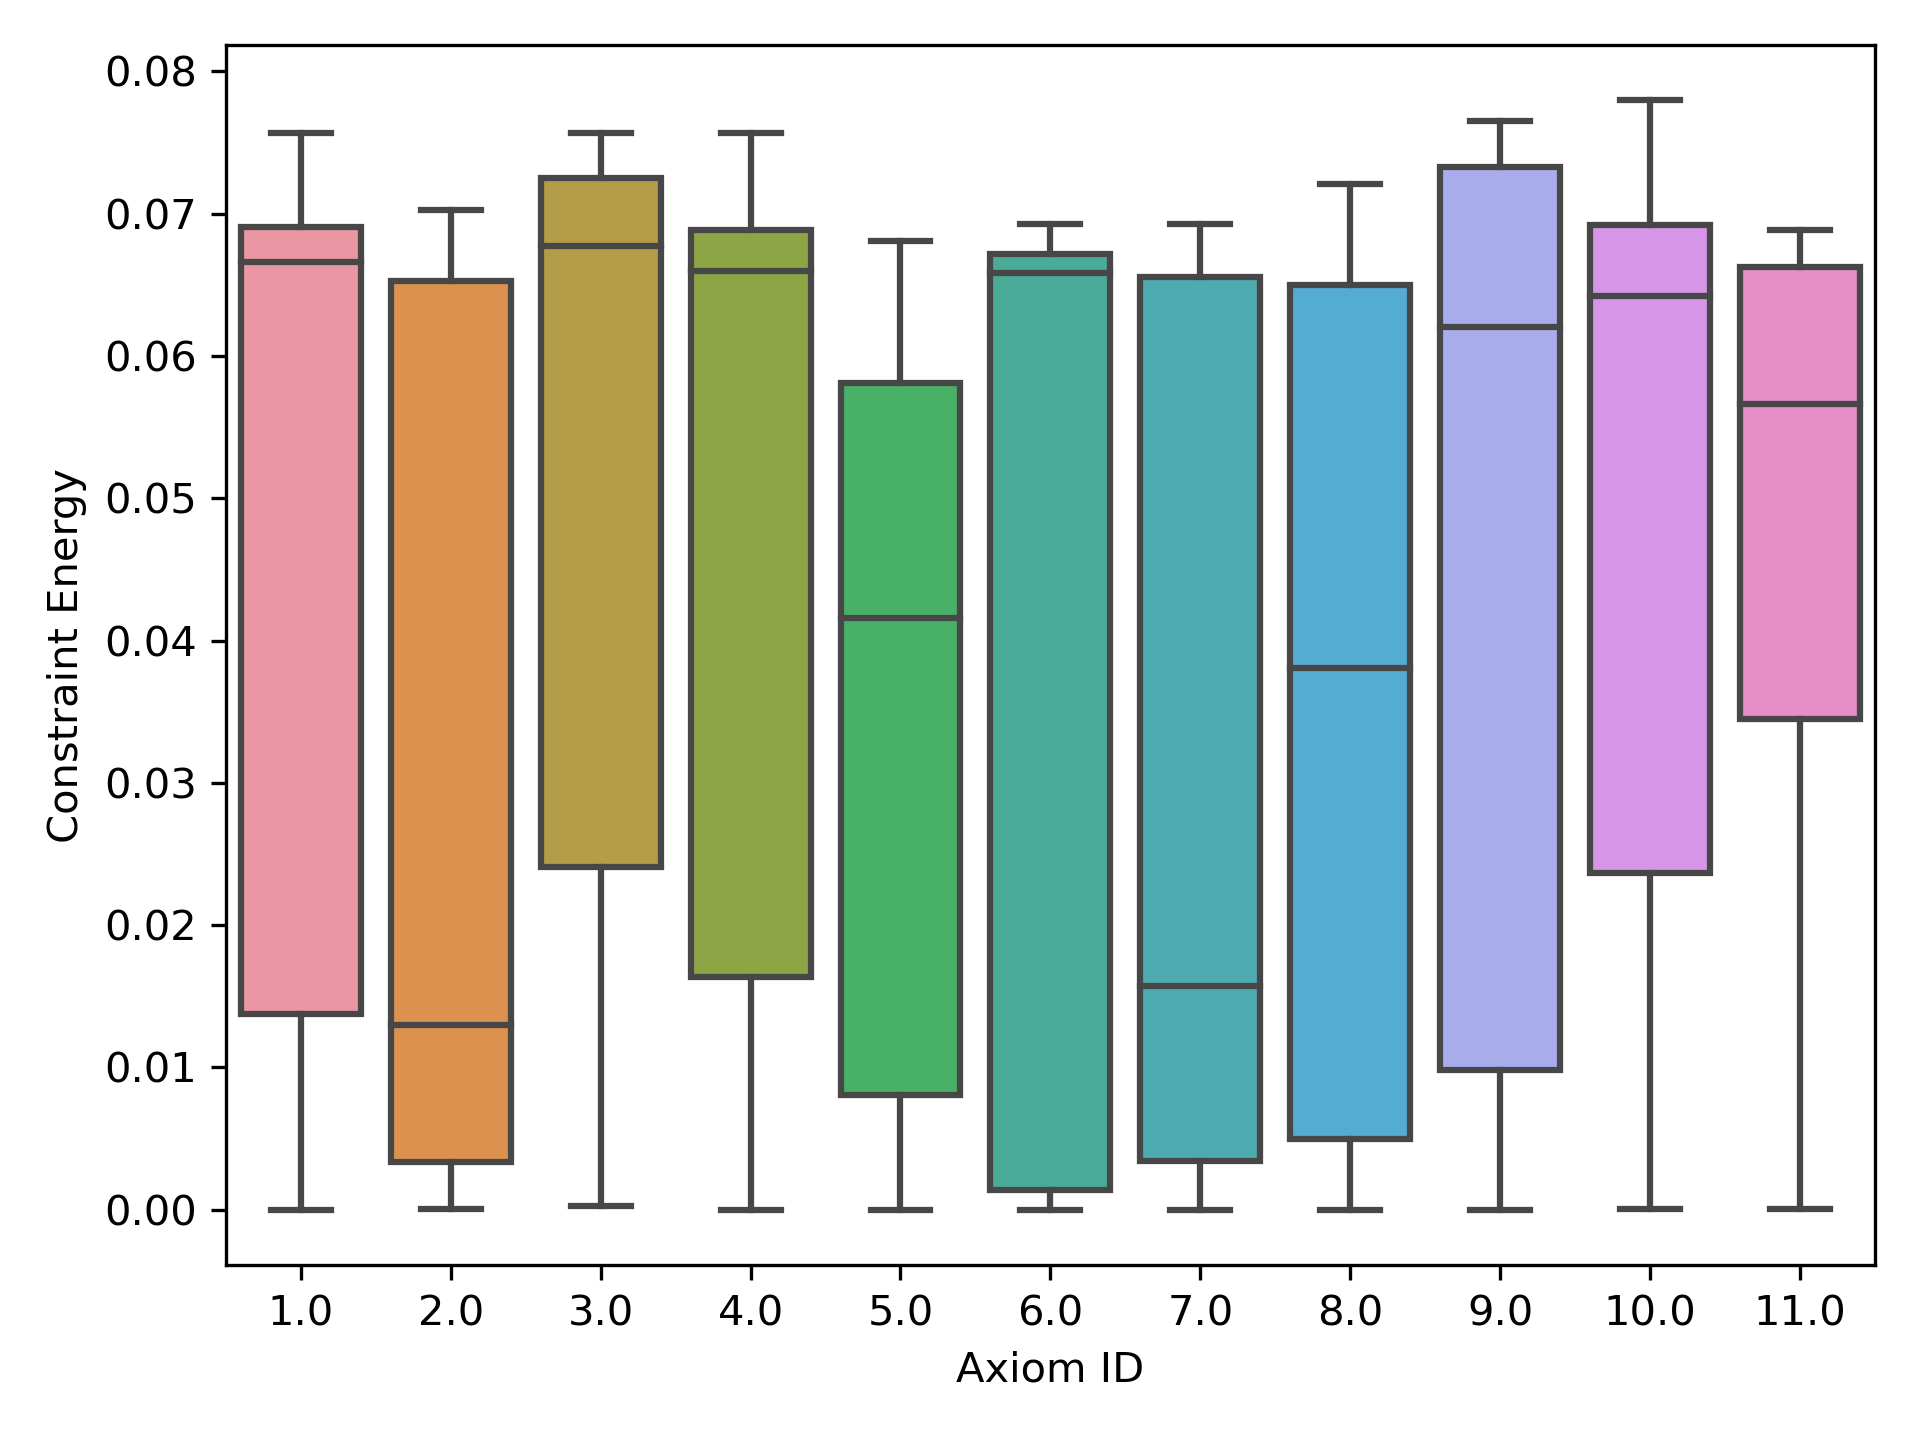
\includegraphics[width=\textwidth]{aid_vs_ce.png}
		\caption{Axiom ID vs constraint energy}
	\end{subfigure}
	\hfill
	\begin{subfigure}[c]{0.45\textwidth}
		\centering
		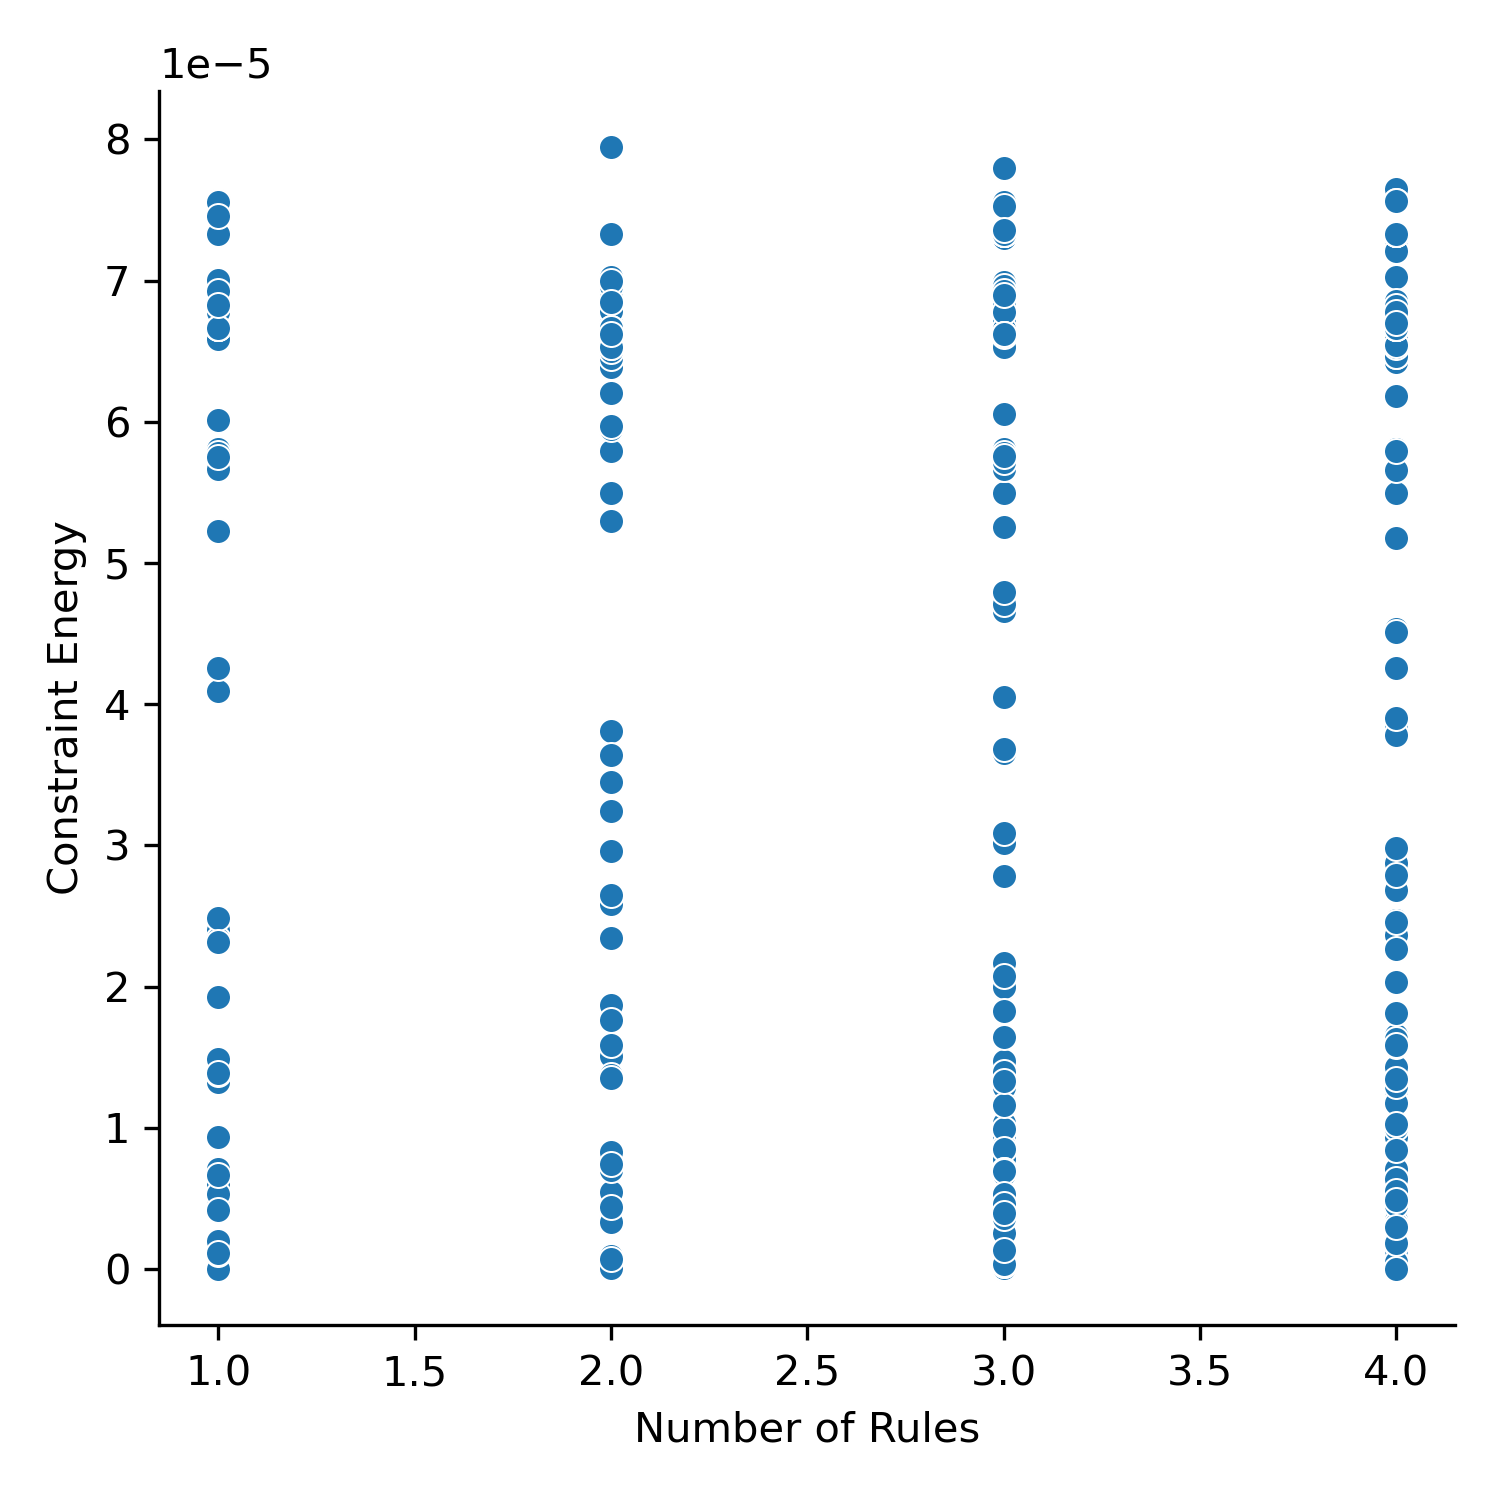
\includegraphics[width=\textwidth]{nor_vs_ce.png}
		\caption{Number of rules vs constraint energy}
	\end{subfigure}
	\hfill
	\begin{subfigure}[c]{0.45\textwidth}
		\centering
		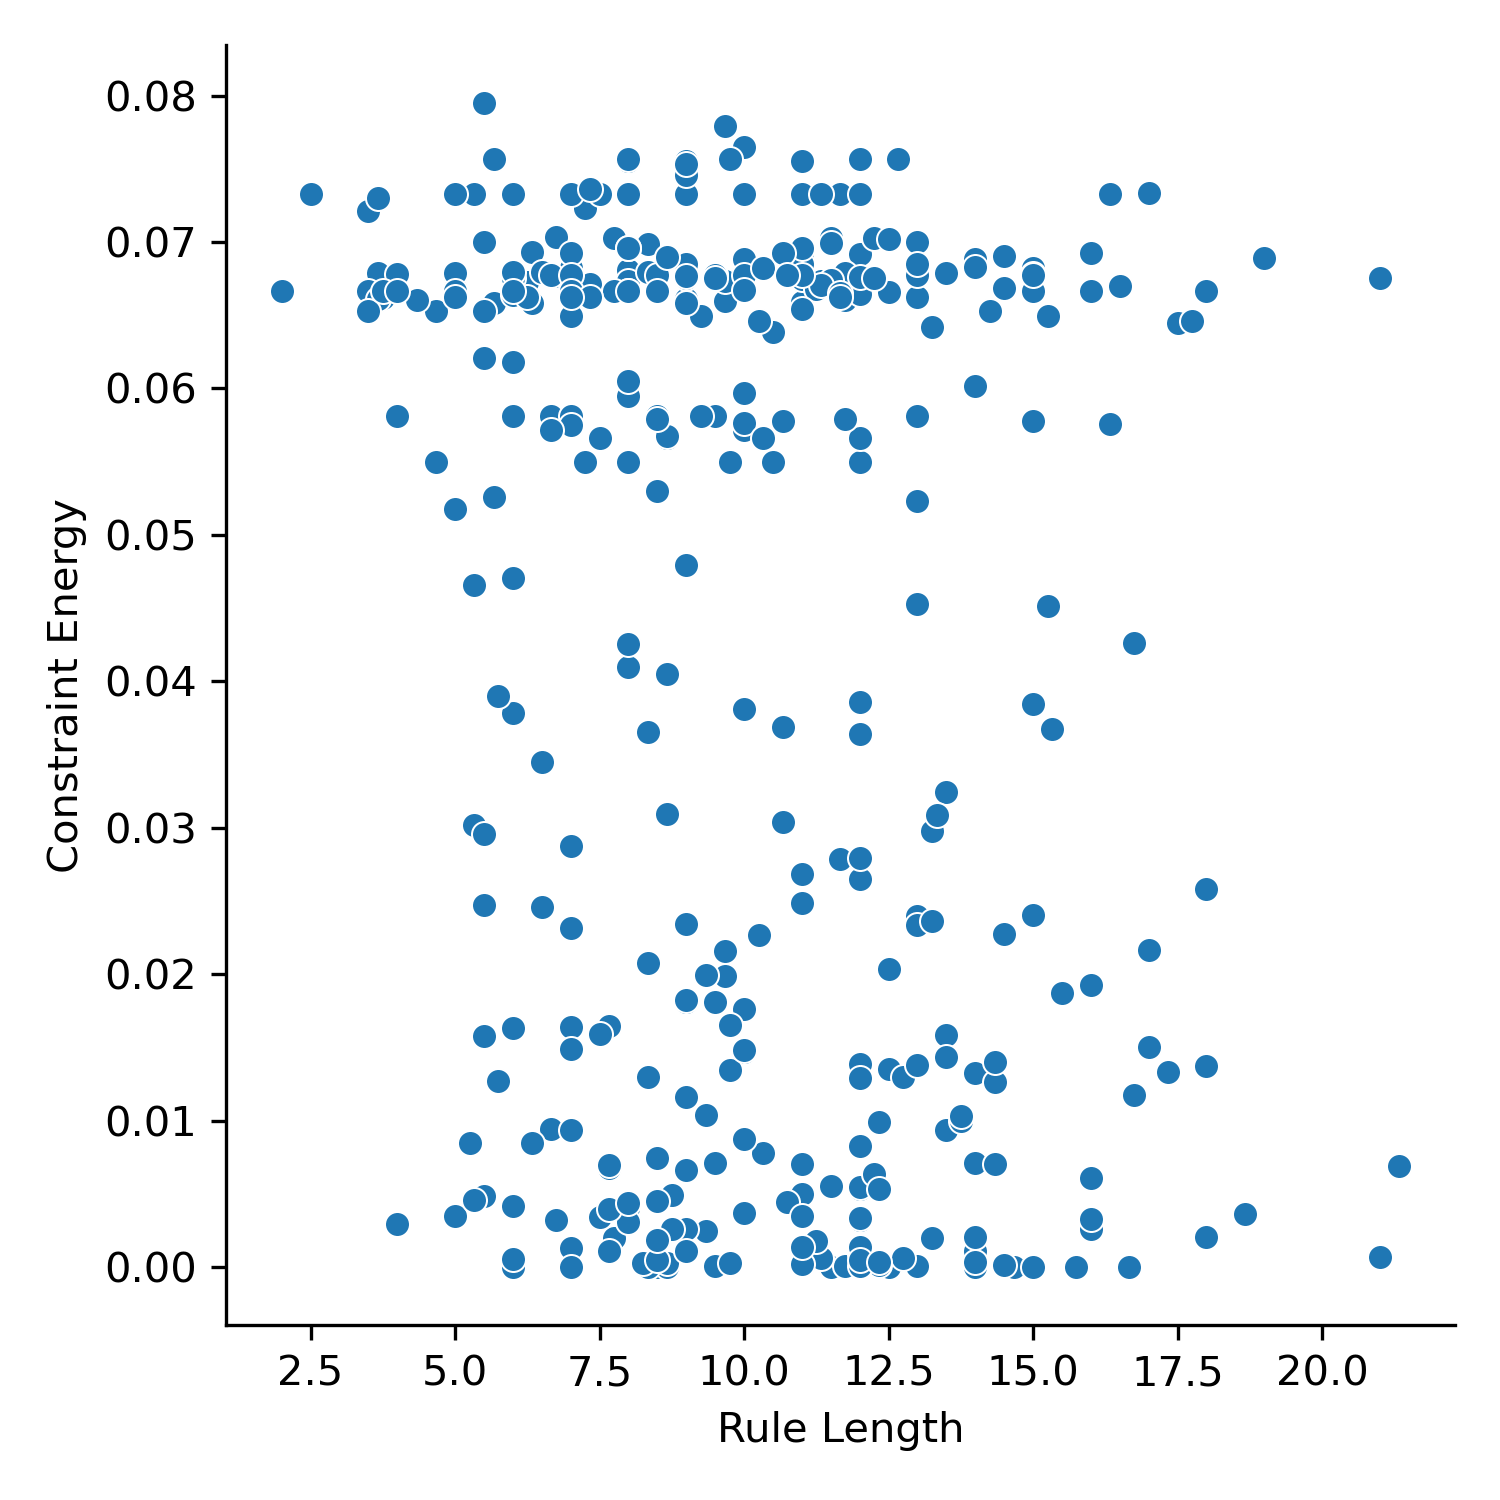
\includegraphics[width=\textwidth]{rl_vs_ce.png}
		\caption{Average rule length vs constraint energy}
	\end{subfigure}
	\hfill
	\begin{subfigure}[c]{0.45\textwidth}
		\centering
		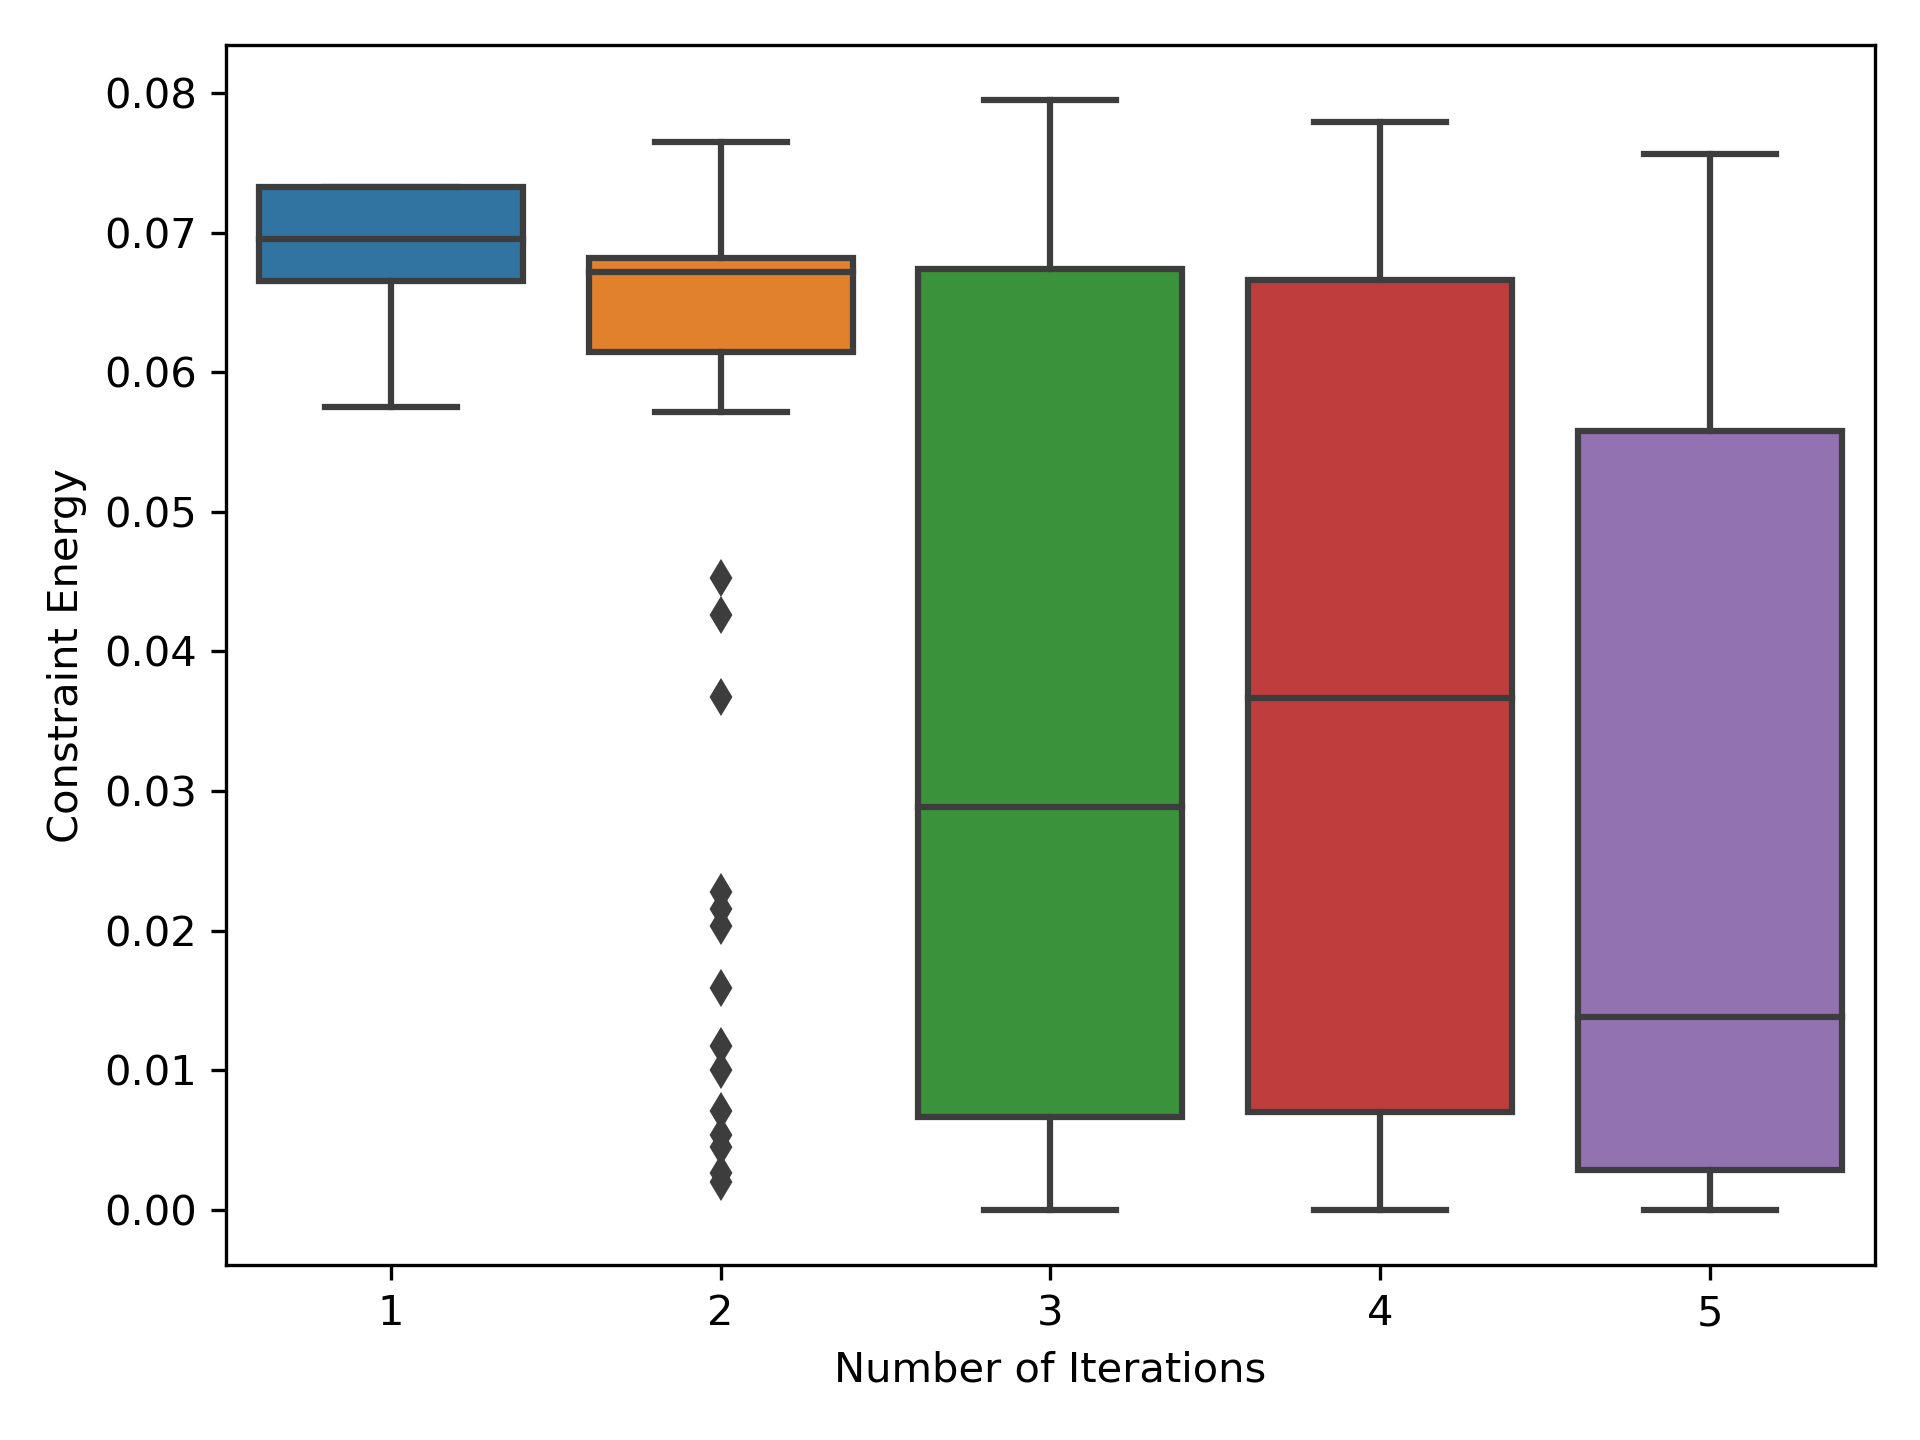
\includegraphics[width=\textwidth]{noi_vs_ce.png}
		\caption{Number of iterations vs constraint energy}
	\end{subfigure}
	\caption[L-System parameters vs constraint energy]{L-System parameters vs constraint energy (\si{mJ}) scatter plots}
	\label{fig:ls_v_ce}
\end{figure}

The L-System parameters have no discernible relationships with the constraint energy. The only exception to the general distribution is in the case of 1 rule iteration, for which the constraint energy is generally high.

Figure~\ref{fig:ls_v_ie} contains scatter plots relating L-System parameters to the constraint energy.

\begin{figure}[H]
	\centering
	\begin{subfigure}[c]{0.45\textwidth}
		\centering
		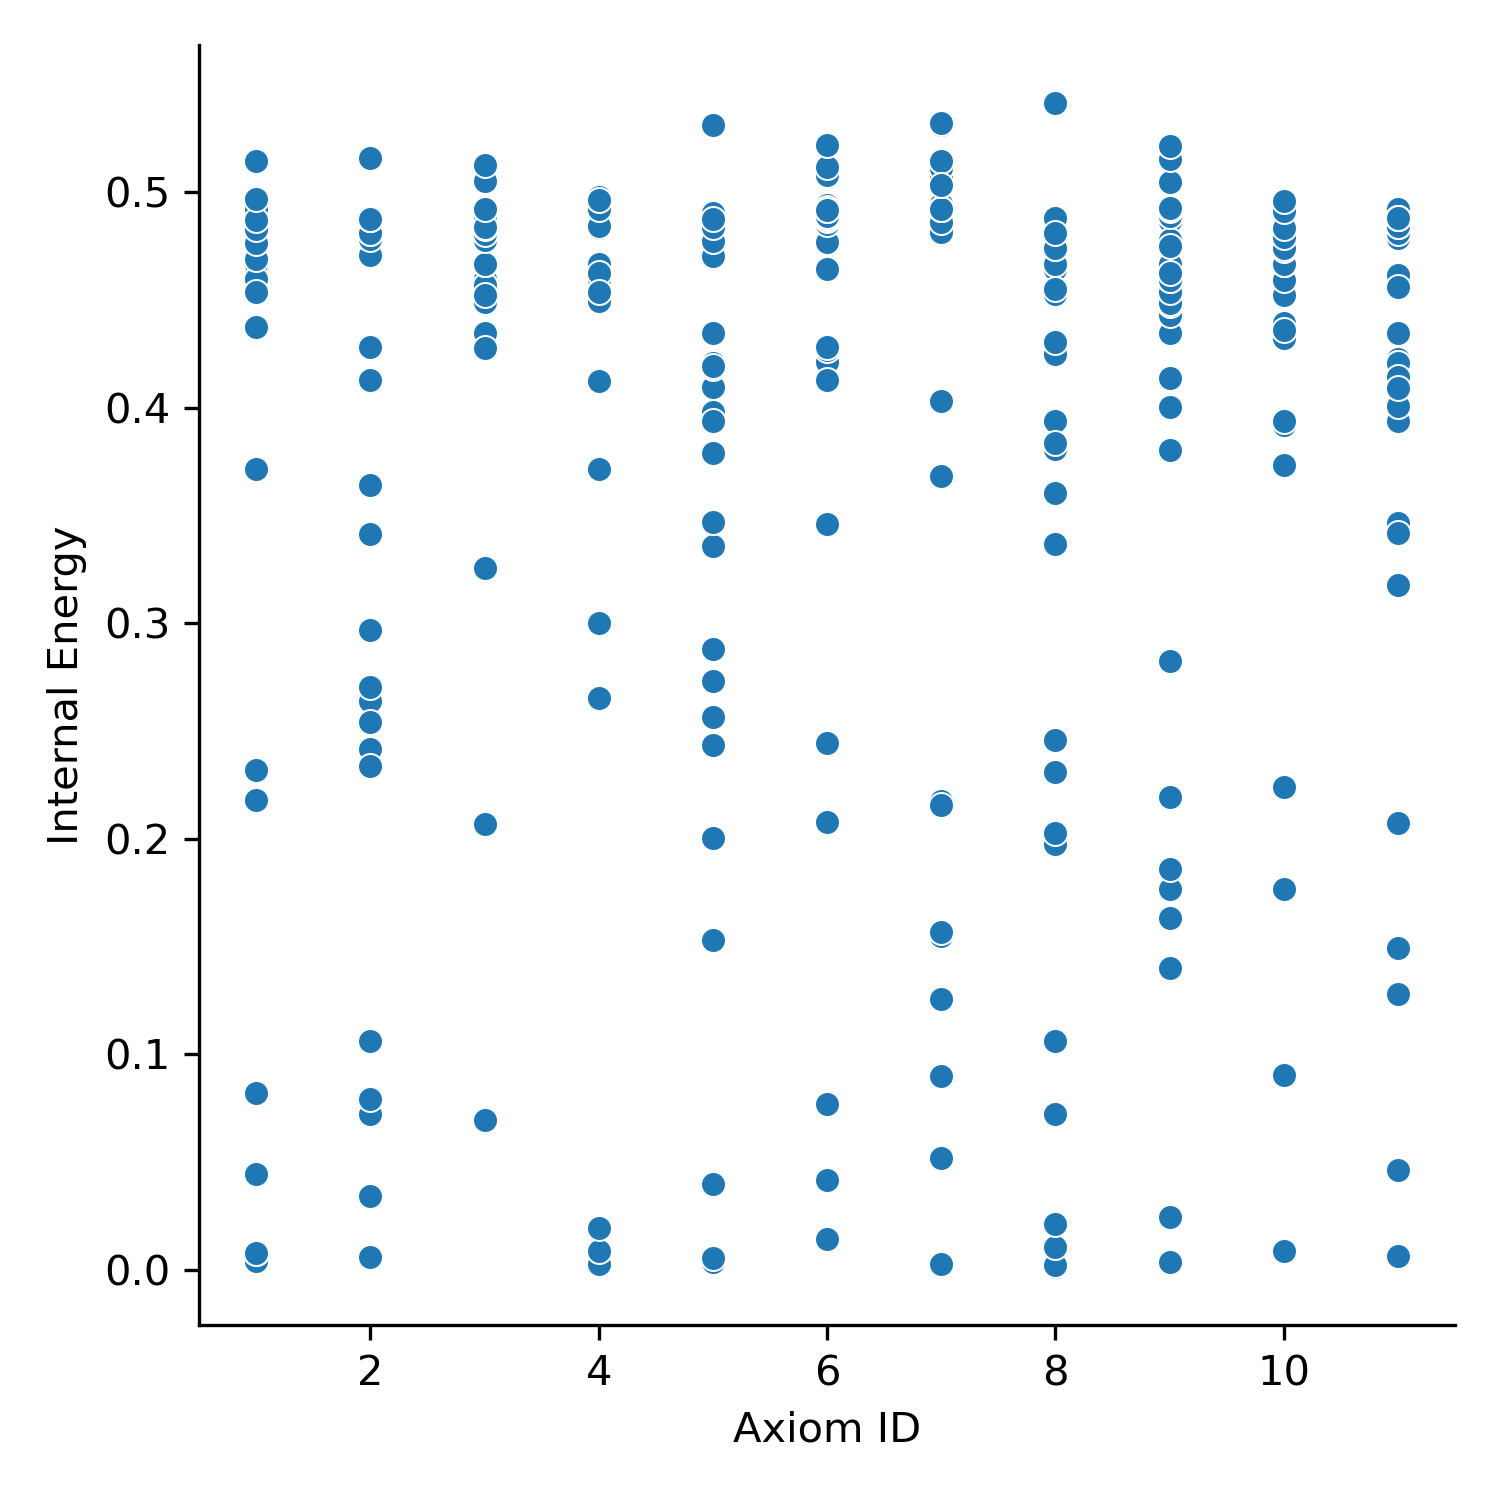
\includegraphics[width=\textwidth]{aid_vs_ie.png}
		\caption{Axiom ID vs internal energy}
	\end{subfigure}
	\hfill
	\begin{subfigure}[c]{0.45\textwidth}
		\centering
		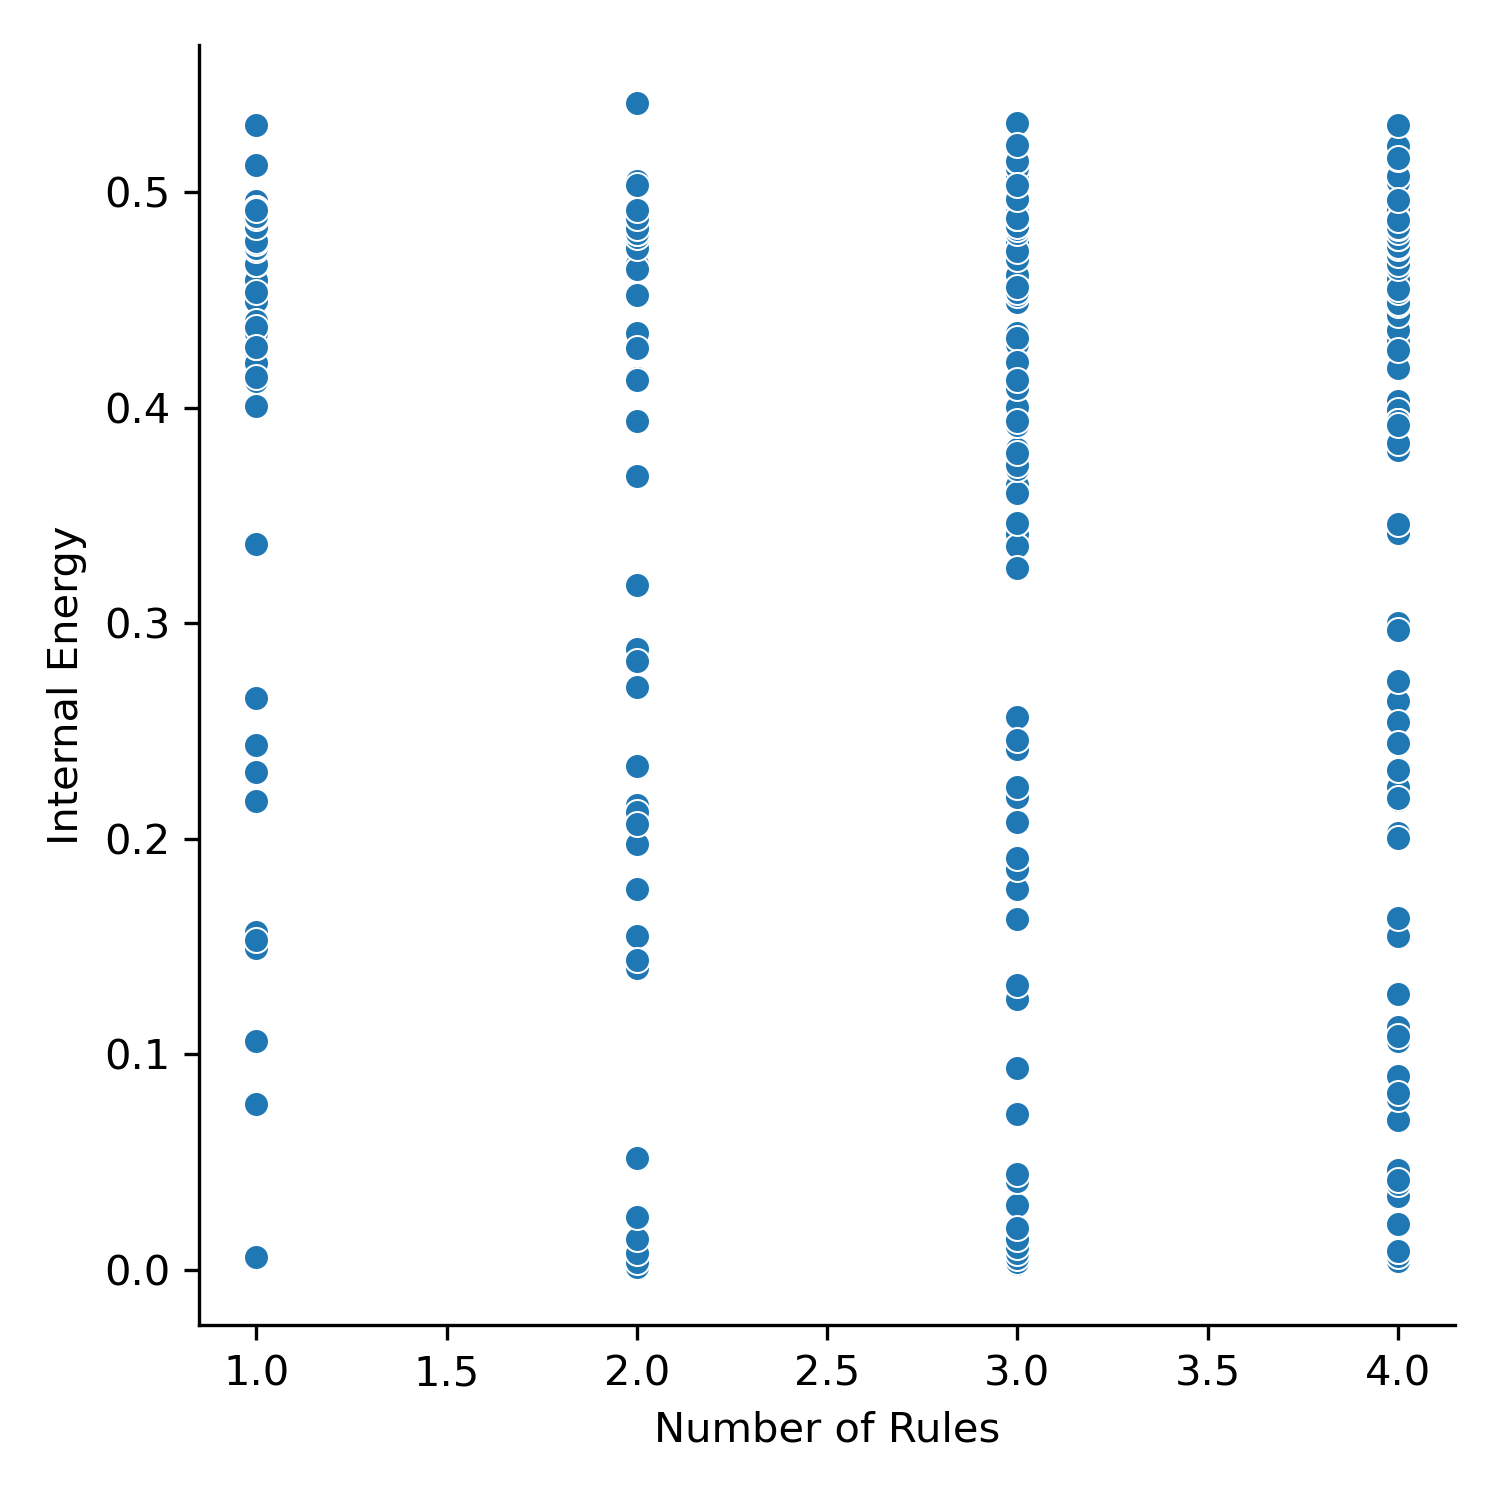
\includegraphics[width=\textwidth]{nor_vs_ie.png}
		\caption{Number of rules vs internal energy}
	\end{subfigure}
	\hfill
	\begin{subfigure}[c]{0.45\textwidth}
		\centering
		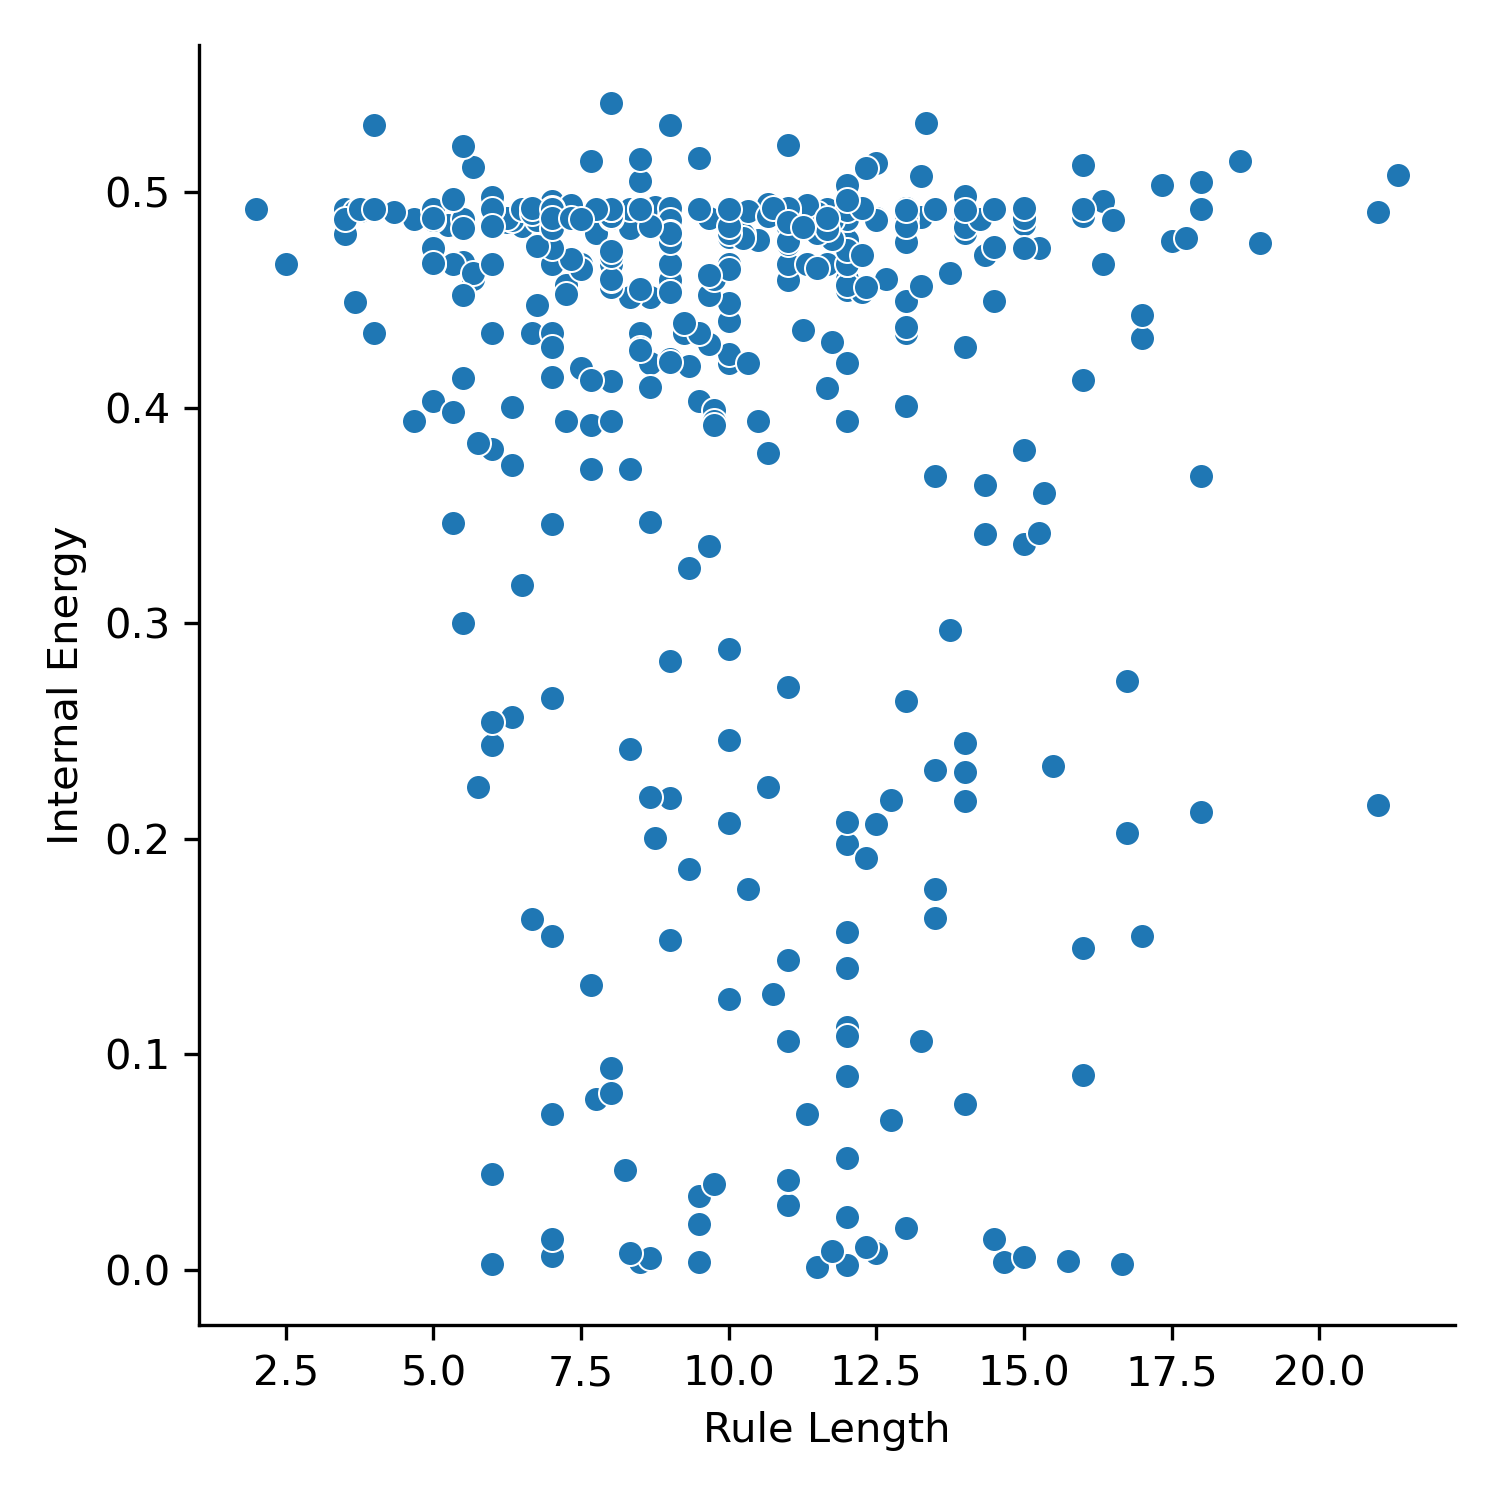
\includegraphics[width=\textwidth]{rl_vs_ie.png}
		\caption{Average rule length vs internal energy}
	\end{subfigure}
	\hfill
	\begin{subfigure}[c]{0.45\textwidth}
		\centering
		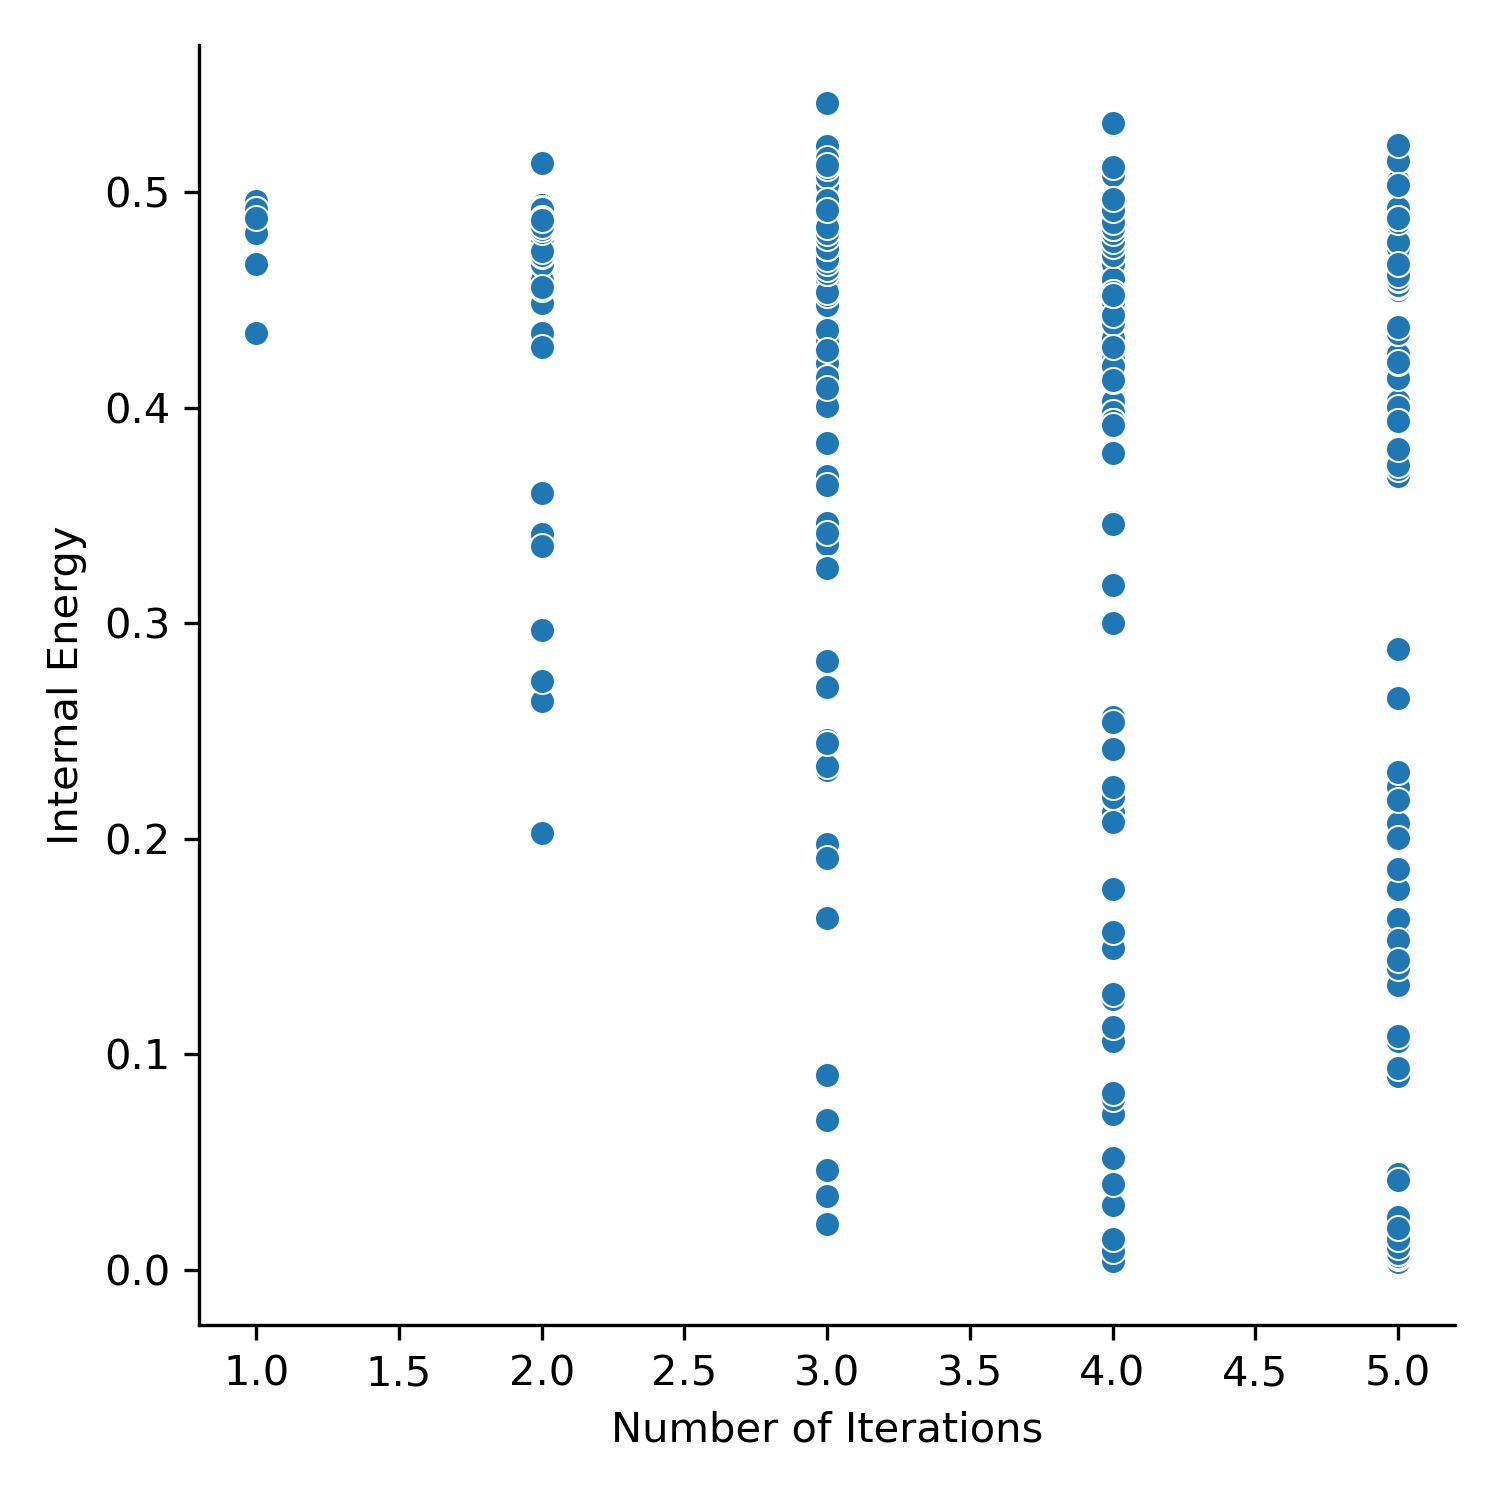
\includegraphics[width=\textwidth]{noi_vs_ie.png}
		\caption{Number of iterations vs internal energy}
	\end{subfigure}
	\caption[L-System parameters vs internal energy]{L-System parameters vs internal energy (\si{mJ}) scatter plots}
	\label{fig:ls_v_ie}
\end{figure}

The L-System parameters have no discernible relationships with the internal energy.

\subsection{CPPN Unit Generation}

Parameter ranges are outlined in Table~\ref{tab:cppnmc}.

% Please add the following required packages to your document preamble:
% \usepackage{booktabs}
\begin{table}[H]
\centering
\caption{CPPN unit generation parameters for a Monte Carlo analysis}
\label{tab:cppnmc}
\begin{tabular}{@{}lcc@{}}
\toprule
\multicolumn{1}{c}{\textbf{Parameter}} & \textbf{Minimum} & \textbf{Maximum} \\ \midrule
Seed                                   & 1                & 1000             \\
Model ID                               & 1                & N/A              \\
Scale                                  & 1                & N/A              \\
Number of hidden layers                & 2                & 10               \\
Size of the initial hidden layer       & 2                & 32               \\
Element removal threshold              & 0                & 100              \\ \bottomrule
\end{tabular}
\end{table}

\subsection{Comparison}

The distribution of the constraint and internal energies for the three unit generation methods is compared in Figure~\ref{fig:ciecomp}.

\begin{figure}[H]
	\centering
	\begin{subfigure}[c]{0.45\textwidth}
		\centering
		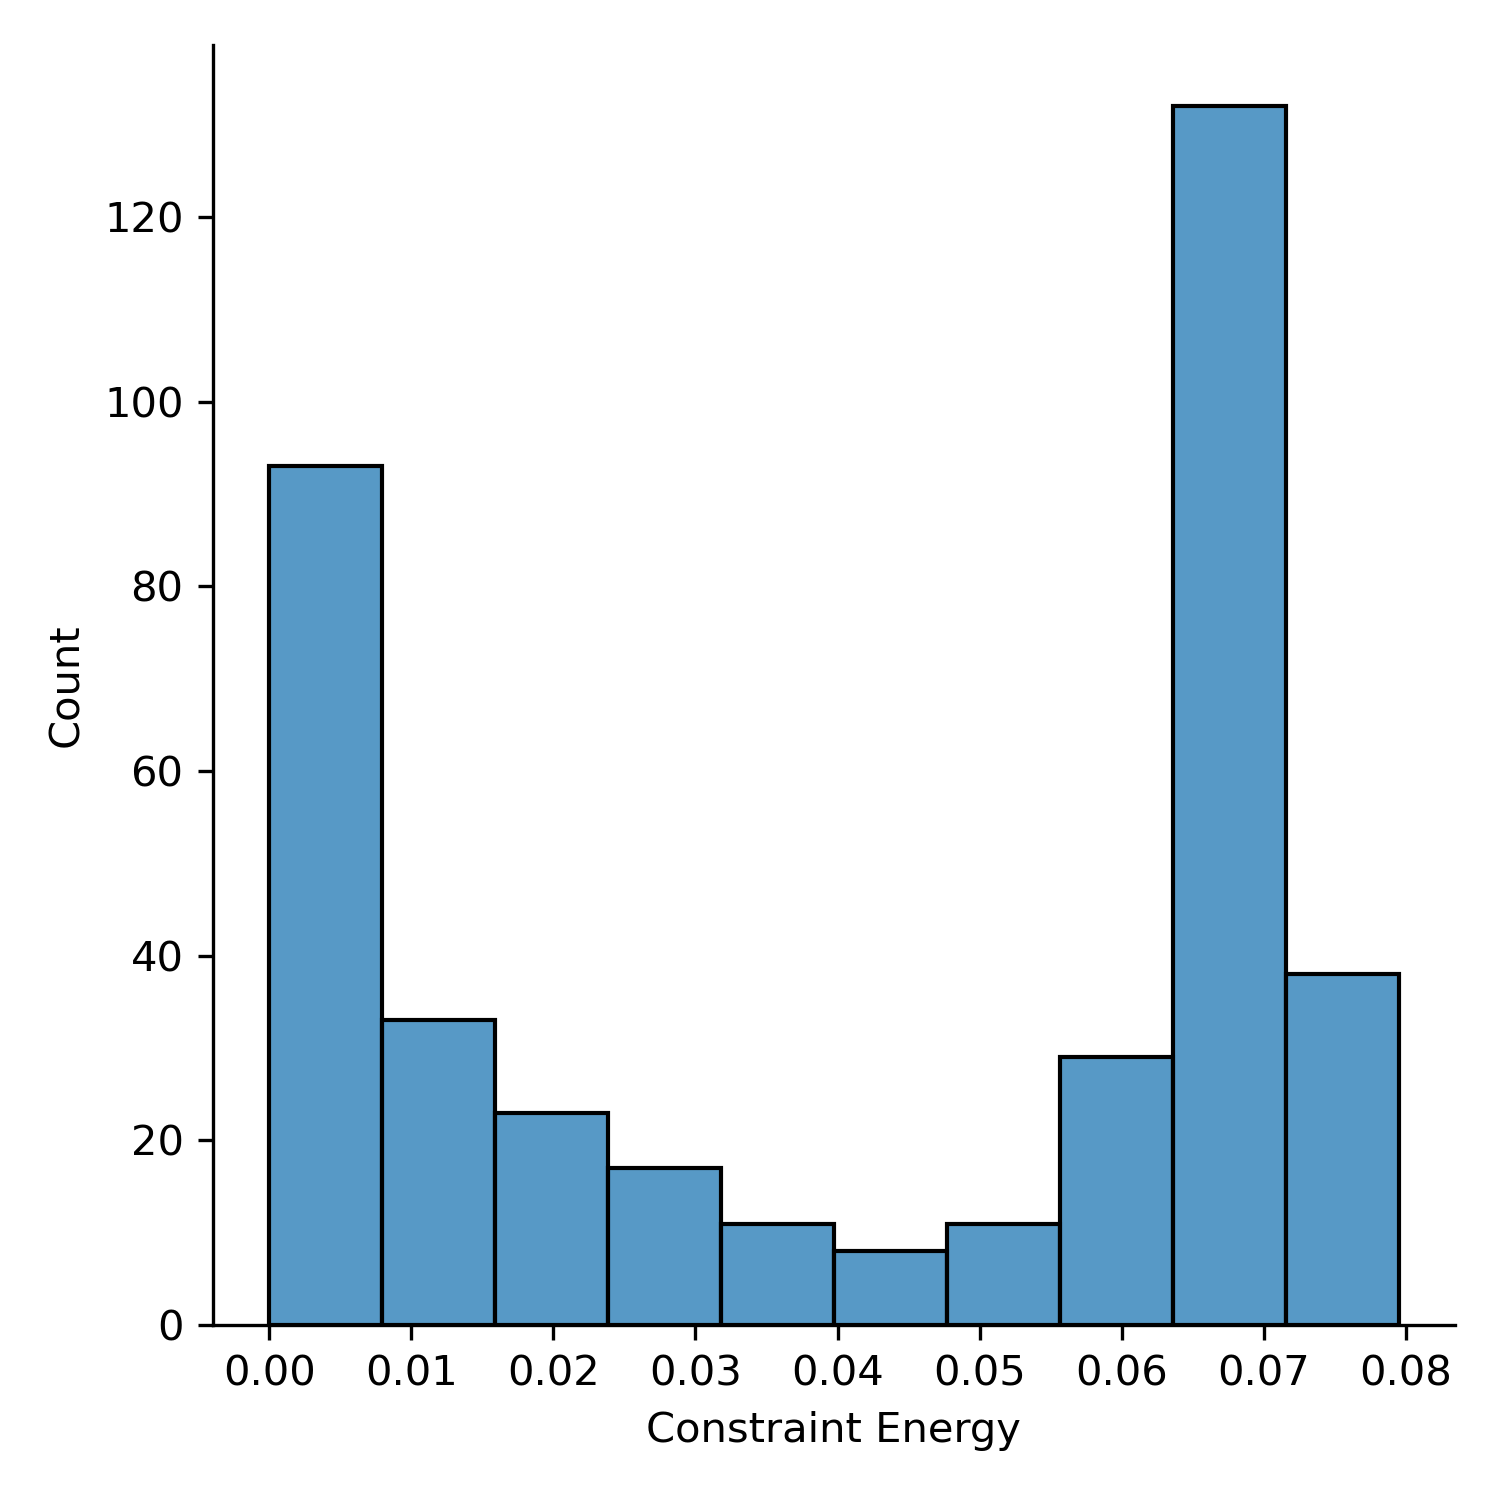
\includegraphics[width=\textwidth]{ce_ls.png}
		\caption{Constraint energy distribution of L-Systems}
	\end{subfigure}
	\hfill
	\begin{subfigure}[c]{0.45\textwidth}
		\centering
		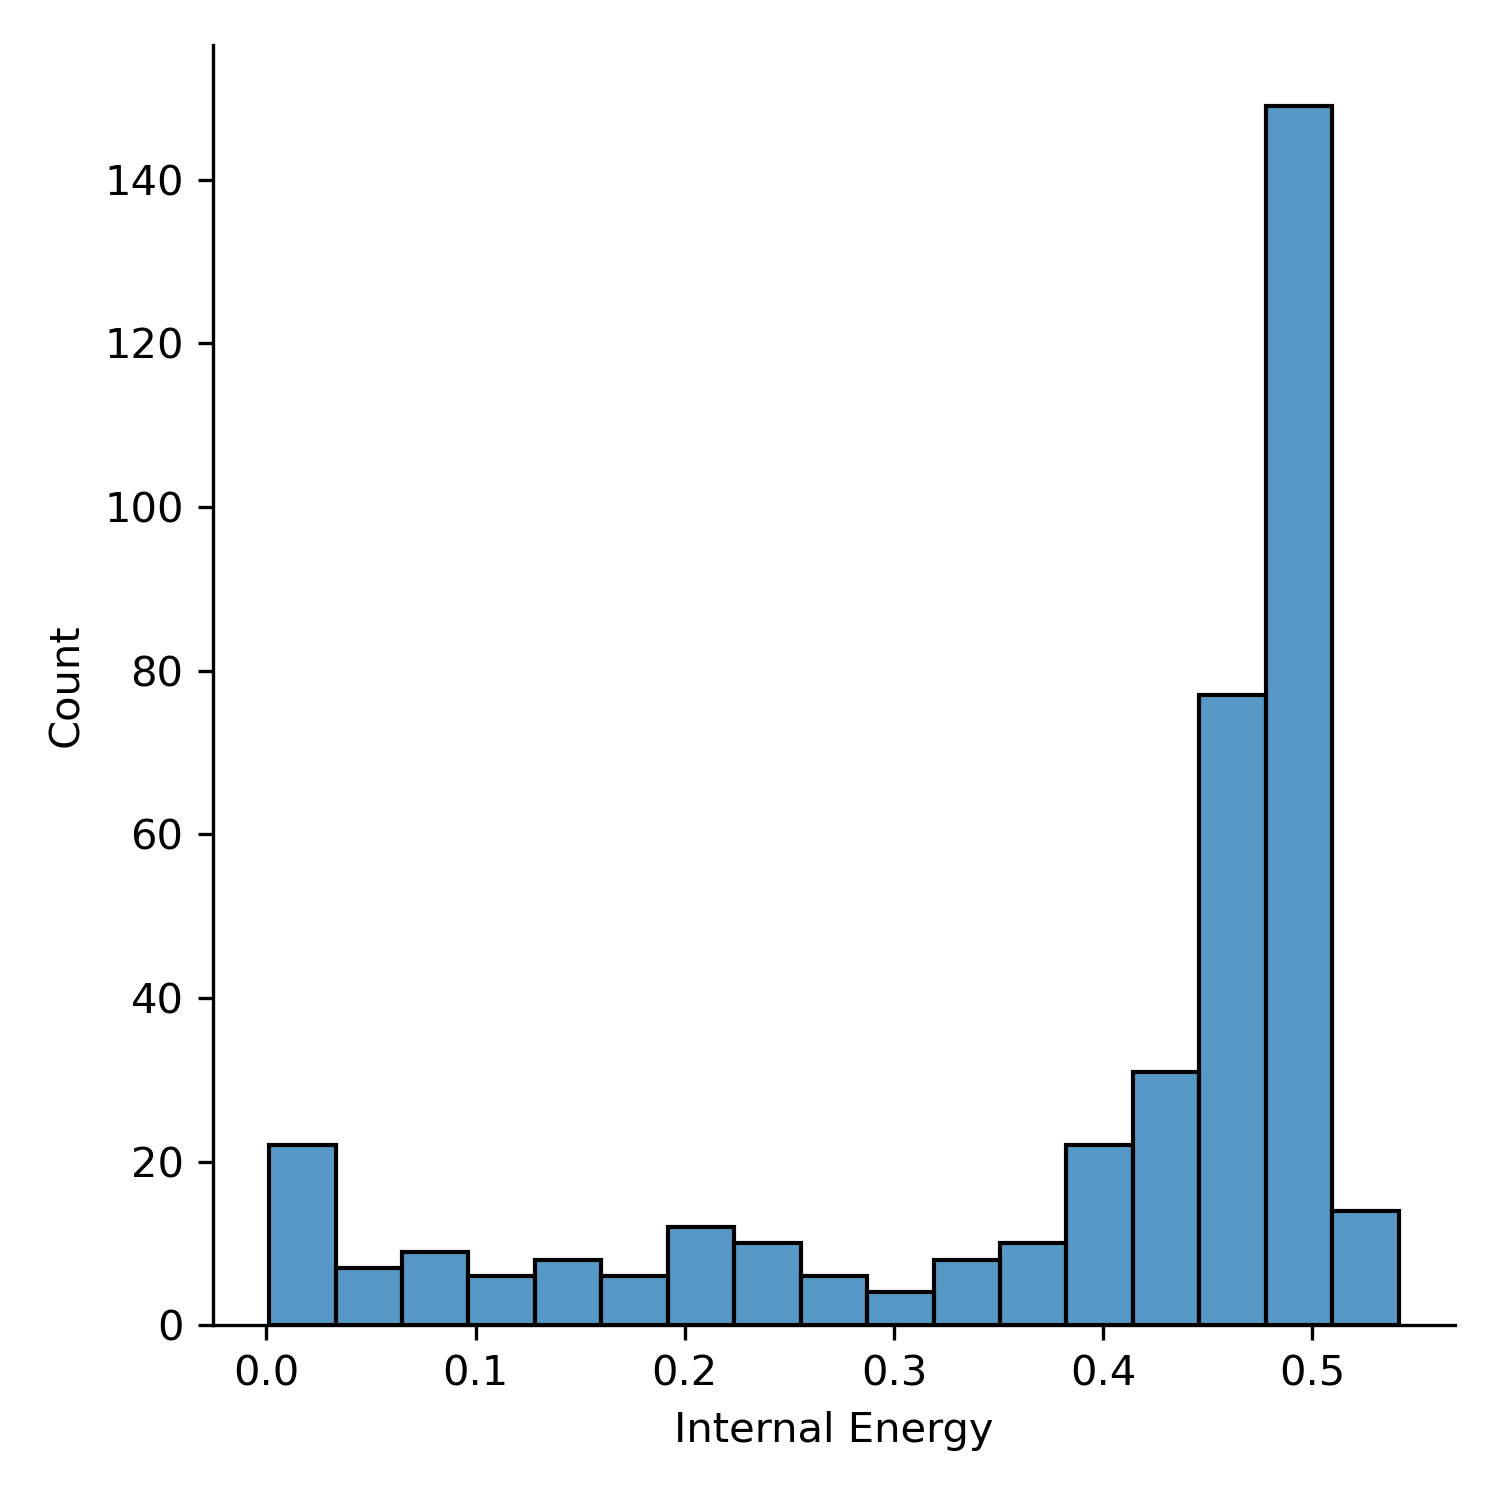
\includegraphics[width=\textwidth]{ie_ls.png}
		\caption{Internal energy distribution of L-Systems}
	\end{subfigure}
	\caption[Constraint and internal energy distribution comparison]{Constraint and internal energy distribution comparison between random, L-System and CPPN unit generation}
	\label{fig:ciecomp}
\end{figure}

\section{Scale Invariance}